% Neighbourhood Stability in Assignments on Graphs -- CS698I paper presentation
% Build: ./build.sh   ->  slides.pdf (projector) and notes.pdf (speaker notes)
\documentclass[aspectratio=169,11pt]{beamer}
\ifdefined\NOTESONLY
  \setbeameroption{show only notes}
\fi
\usepackage[T1]{fontenc}
\usepackage{lmodern}
\usepackage{amsmath,amssymb}
\usepackage{booktabs}
\usepackage{tikz}
\usetikzlibrary{arrows.meta,positioning,calc,decorations.pathreplacing}

% ---------- colours ----------
\definecolor{ink}{HTML}{1F2933}
\definecolor{accent}{HTML}{0B5394}
\definecolor{warn}{HTML}{C0392B}
\definecolor{good}{HTML}{1E8449}
\definecolor{muted}{HTML}{6B7280}
\definecolor{linkbg}{HTML}{E8F0FA}
\definecolor{viewbg}{HTML}{FDF0E6}
\definecolor{Afill}{HTML}{BFE3F8}\definecolor{Adraw}{HTML}{0072B2}
\definecolor{Bfill}{HTML}{FBE0A8}\definecolor{Bdraw}{HTML}{B87A00}
\definecolor{Cfill}{HTML}{B8E6D3}\definecolor{Cdraw}{HTML}{007A58}
\definecolor{Dfill}{HTML}{F2C9DF}\definecolor{Ddraw}{HTML}{A64D84}

% ---------- beamer look ----------
\setbeamertemplate{navigation symbols}{}
\setbeamercolor{normal text}{fg=ink,bg=white}
\setbeamercolor{frametitle}{fg=accent}
\setbeamerfont{frametitle}{series=\bfseries,size=\Large}
\setbeamercolor{structure}{fg=accent}
\setbeamertemplate{itemize items}{\color{accent}\raisebox{0.15ex}{\small$\blacktriangleright$}}
\setbeamertemplate{enumerate items}[default]
\setbeamerfont{title}{series=\bfseries,size=\LARGE}
\def\who{}
\setbeamertemplate{footline}{%
  \hfill{\scriptsize\color{muted}\who\quad\insertframenumber\,/\,\inserttotalframenumber}\hspace*{5mm}\vspace*{2.5mm}}
\setbeamertemplate{note page}{%
  \vspace*{2mm}%
  \begin{minipage}[t]{0.22\textwidth}\vspace{0pt}\insertslideintonotes{0.2}\end{minipage}%
  \hfill
  \begin{minipage}[t]{0.76\textwidth}\vspace{0pt}\small\raggedright\insertnote\end{minipage}}

% ---------- notation ----------
\newcommand{\nlikes}{\nrightarrow}
\newcommand{\NS}{neighbourhood stable}
\newcommand{\tm}[3]{\textbf{\color{accent}[#1 \textperiodcentered{} #2 \textperiodcentered{} ends at #3]}\par\smallskip}
\newcommand{\idea}[1]{\par\medskip\noindent\colorbox{linkbg}{\parbox{\dimexpr\linewidth-2\fboxsep}{\centering #1}}}
\newcommand{\ourview}[1]{\par\smallskip\noindent\colorbox{viewbg}{\parbox{\dimexpr\linewidth-2\fboxsep}{\small\textbf{\color{warn}Our view.} #1}}}
\newcommand{\src}[1]{{\scriptsize\color{muted}#1}}

% ---------- tikz styles ----------
\tikzset{
  ag/.style={circle,draw,thick,minimum size=7.5mm,inner sep=0pt,font=\bfseries},
  aga/.style={ag,fill=Afill,draw=Adraw}, agb/.style={ag,fill=Bfill,draw=Bdraw},
  agc/.style={ag,fill=Cfill,draw=Cdraw}, agd/.style={ag,fill=Dfill,draw=Ddraw},
  agg/.style={ag,fill=gray!12,draw=gray!60!black,font=\small},
  sm/.style={circle,draw,thick,minimum size=6mm,inner sep=0pt,font=\small},
  arc/.style={-{Stealth[length=2.4mm]},thick,draw=ink!85},
  like/.style={-{Stealth[length=2.4mm]},thick,draw=good},
  bad/.style={-{Stealth[length=2.4mm]},thick,draw=warn},
  sedge/.style={line width=1.4pt,draw=gray!55},
  hot/.style={line width=4pt,draw=warn!80},
  lab/.style={font=\scriptsize,text=muted},
  ut/.style={font=\small\bfseries,text=accent},
}
% Fig. 2 preference graph (a<->c, b<->d, b->a, d->c)
\newcommand{\figtwopref}{%
  \node[aga] (a) at (0,1.7) {a}; \node[agc] (c) at (2.2,1.7) {c};
  \node[agb] (b) at (0,0) {b};   \node[agd] (d) at (2.2,0) {d};
  \draw[arc] (a) to[bend left=18] (c); \draw[arc] (c) to[bend left=18] (a);
  \draw[arc] (b) to[bend left=18] (d); \draw[arc] (d) to[bend left=18] (b);
  \draw[arc] (b) -- (a); \draw[arc] (d) -- (c);}
% Fig. 6 preference graph (c->a, a->b, a->d, b->d, d->c)
\newcommand{\figsixpref}{%
  \node[aga] (a) at (0,1.7) {a}; \node[agc] (c) at (2.2,1.7) {c};
  \node[agb] (b) at (0,0) {b};   \node[agd] (d) at (2.2,0) {d};
  \draw[arc] (c) -- (a); \draw[arc] (a) -- (b); \draw[arc] (a) -- (d);
  \draw[arc] (b) -- (d); \draw[arc] (d) -- (c);}
% four agents on a path of seats v1..v4
\newcommand{\pathseat}[4]{%
  \draw[sedge] (0,0) -- (4.8,0);
  \node[ag#1] (#1) at (0,0) {#1}; \node[ag#2] (#2) at (1.6,0) {#2};
  \node[ag#3] (#3) at (3.2,0) {#3}; \node[ag#4] (#4) at (4.8,0) {#4};}
\newcommand{\seatlabels}{\foreach \i in {1,...,4}{\node[lab] at ({(\i-1)*1.6},-0.62) {$v_{\i}$};}}
% four agents on a 4-cycle of seats (TL, TR, BR, BL = v1..v4); #5,#6 = highlighted pair
\newcommand{\sqseat}[6]{%
  \coordinate (#1) at (0,1.4); \coordinate (#2) at (1.4,1.4);
  \coordinate (#3) at (1.4,0); \coordinate (#4) at (0,0);
  \draw[sedge] (#1)--(#2)--(#3)--(#4)--cycle;
  \draw[hot] (#5)--(#6);
  \node[ag#1] (#1) at (#1) {#1}; \node[ag#2] (#2) at (#2) {#2};
  \node[ag#3] (#3) at (#3) {#3}; \node[ag#4] (#4) at (#4) {#4};}

\title{Neighborhood Stability in Assignments on Graphs}
\author{Ashik Stenny (230224) \quad\textperiodcentered\quad Achyuth H Warrier (230052)}
\date{11 November 2026}

\begin{document}

% =====================================================================
\def\who{}
% ---------------------------------------------------------------- 1
\begin{frame}[plain]
  \vspace*{6mm}
  {\color{accent}\LARGE\bfseries Neighborhood Stability in\\[1mm] Assignments on Graphs\par}
  \vspace{3mm}
  {\large Haris Aziz, Grzegorz Lisowski, Mashbat Suzuki, Jeremy Vollen\par}
  {\small\color{muted} arXiv:2407.05240, 2024\par}
  \vspace{8mm}
  {\large Presented by Ashik Stenny (230224) and Achyuth H Warrier (230052)\par}
  \vspace{2mm}
  {\small\color{muted}CS698I: Relational Structures in Games \textperiodcentered{} IIT Kanpur \textperiodcentered{} Instructor: Sunil Simon\\ 11 November 2026\par}
\note{\tm{Ashik}{0:30}{0:30}
Good morning. We are presenting ``Neighborhood Stability in Assignments on Graphs'' by Aziz, Lisowski, Suzuki and Vollen, posted on arXiv in 2024.

I will do the first half: the model, why stability can fail, and why letting people swap does not always work. Achyuth will do the second half: the algorithms that \emph{do} work on cycles, paths, and a general family of graphs.

Throughout, we will use one story (a dinner party) and one small four-guest example.}
\end{frame}

% ---------------------------------------------------------------- 2
\begin{frame}{The dinner-party problem}
\begin{columns}[T]
\column{0.38\textwidth}
\centering
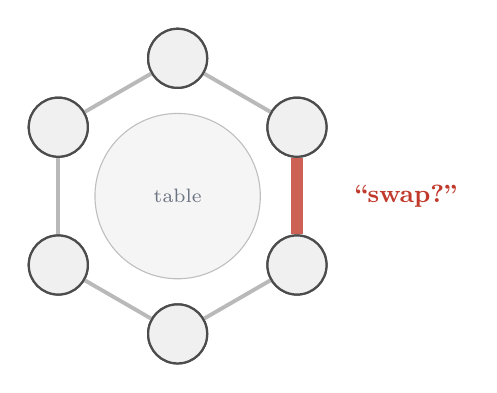
\begin{tikzpicture}[scale=1]
  \draw[fill=gray!8,draw=gray!50] (0,0) circle (1.05);
  \node[lab] at (0,0) {table};
  \foreach \ang/\n in {90/1,30/2,-30/3,-90/4,-150/5,150/6}{\node[agg] (g\n) at (\ang:1.75) {};}
  \foreach \i/\j in {1/2,2/3,3/4,4/5,5/6,6/1}{\draw[sedge] (g\i)--(g\j);}
  \draw[hot] (g2)--(g3);
  \foreach \ang/\n in {90/1,30/2,-30/3,-90/4,-150/5,150/6}{\node[agg] at (\ang:1.75) {};}
  \node[font=\small\bfseries,text=warn,align=center] at (2.9,0) {``swap?''};
\end{tikzpicture}
\column{0.6\textwidth}
\begin{itemize}\setlength\itemsep{2mm}
  \item A host seats $n$ guests on $n$ fixed seats.
  \item Each guest \textbf{likes} some of the others: a yes/no list.
  \item Happiness = how many liked guests sit \textbf{next to you}.
  \item Two neighbours who would \emph{both} be happier after swapping seats will swap.
\end{itemize}
\vspace{3mm}
{\large\bfseries Goal: a seating where no two neighbours want to swap.}
\end{columns}
\note{\tm{Ashik}{0:45}{1:15}
Imagine you are hosting a dinner. Seats are fixed. Each guest has a simple yes/no opinion of every other guest: either they like them or they don't. A guest's happiness is just the number of liked guests sitting next to them.

Now the trouble: if two guests sitting next to each other would \emph{both} be happier after swapping seats, they will lean over, agree, and swap. Then others may want to swap, and so on.

The host wants to avoid this: find a seating in which no two neighbours want to swap.

(The paper's introduction tells the same story with an organisation assigning members to roles; the dinner party is the version from the earlier literature, Bodlaender et al.)}
\end{frame}

% ---------------------------------------------------------------- 2b
\begin{frame}{Why study this?}
\begin{columns}[T]
\column{0.48\textwidth}
\textbf{\color{accent}Where the problem appears}
\begin{itemize}\setlength\itemsep{2mm}
  \item \textbf{Roles in an organisation:} members don't mind which project they get, only which colleagues they work with.
  \item \textbf{Seating arrangements} (Bodlaender et al.\ 2020) and several follow-up papers.
  \item A relative of \textbf{hedonic games}: agents care only about \emph{who} they are grouped with.
\end{itemize}
\column{0.48\textwidth}
\textbf{\color{accent}Why a new notion of stability}
\begin{itemize}\setlength\itemsep{2mm}
  \item Full stability often fails: Berriaud et al.\ found many non-existence results on paths and cycles.
  \item Precedent: in Schelling games, allowing only \textbf{local swaps} makes equilibria exist on more graphs (Bil\`o et al.).
  \item A swap needs the two agents to interact, so only neighbours can arrange one.
\end{itemize}
\end{columns}
\vspace{4mm}
\small\textbf{Binary preferences} = each agent approves a set of others, as studied in committee voting, matching and item allocation.
\note{\tm{Ashik}{1:00}{2:15}
Why should we care? The paper opens with an organisation example: roles are fixed in advance, members are happy with any project, but they care about which colleagues they work with. If two members would both rather swap roles, you get chaos. The same model was first studied for seating guests, by Bodlaender et al., and several recent papers followed.

It's also closely related to hedonic games, where agents are partitioned into groups and only care about who is in their group.

Why a new stability notion? In hedonic games and in this seating model, stable outcomes often don't exist; Berriaud et al.\ found many non-existence results even on paths and cycles. A similar issue arose in Schelling segregation games, and Bil\`o et al.\ showed that allowing only local swaps makes equilibria exist on more graph classes. That's the inspiration here: only neighbours can swap, which is also realistic, since a swap needs the two people to talk.

Binary preferences, approve or not, are a standard model in committee voting, matching and fair division.}
\end{frame}

% ---------------------------------------------------------------- 3
\begin{frame}{The question the paper asks}
\begin{center}
\begin{minipage}{0.85\textwidth}
\large\itshape ``For which classes of seat graphs is a neighborhood stable assignment guaranteed to exist under binary preferences?''
\end{minipage}
\end{center}
\vspace{6mm}
\begin{columns}[T]
\column{0.47\textwidth}
\textbf{\color{accent}Setting the scene}
\begin{itemize}
  \item The model, on a 4-guest example
  \item Stability can fail
  \item Letting guests swap can loop forever
\end{itemize}
\column{0.47\textwidth}
\textbf{\color{accent}Positive results}
\begin{itemize}
  \item Round tables (cycles): always solvable
  \item Long benches (paths)
  \item A general condition; discussion
\end{itemize}
\end{columns}
\note{\tm{Ashik}{0:30}{2:45}
This is the question the paper asks, quoted directly. ``Seat graph'' is the shape of the table; ``binary preferences'' means the yes/no likes.

Plan: I'll set up the model on a small example, show that a good seating need not exist, and show that letting guests fix things themselves can cycle forever. Achyuth then shows the positive results: on a round table (a cycle) a good seating always exists and can be computed fast; similar for a bench (a path); and a general condition for other seat graphs.}
\end{frame}

% ---------------------------------------------------------------- 4
\begin{frame}{Two graphs: who likes whom, and who sits where}
\begin{columns}[T]
\column{0.42\textwidth}
\centering
\textbf{Preference graph $\mathcal{P}$} (directed)\\[3mm]
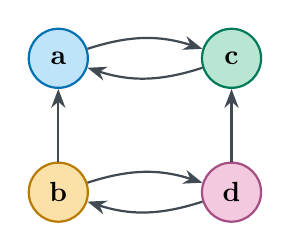
\begin{tikzpicture}\figtwopref\end{tikzpicture}\\[3mm]
{\small $i\to j$: guest $i$ likes guest $j$}
\column{0.55\textwidth}
\centering
\textbf{Seat graph $G$} (undirected)\\[8mm]
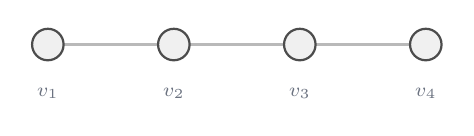
\begin{tikzpicture}
  \draw[sedge] (0,0)--(4.8,0);
  \foreach \i in {1,...,4}{\node[agg,minimum size=4mm] at ({(\i-1)*1.6},0) {};}
  \seatlabels
\end{tikzpicture}\\[6mm]
{\small edge = the two seats are next to each other}
\end{columns}
\vspace{6mm}
\begin{itemize}
  \item An \textbf{assignment} $\pi$ puts each of the $n$ agents on one of the $n$ seats (a bijection).
  \item \textbf{Running example} (paper's Fig.~2): $a\leftrightarrow c$, $b\leftrightarrow d$, $b\to a$, $d\to c$; seats in a row.
\end{itemize}
\note{\tm{Ashik}{1:30}{4:15}
There are two separate graphs here, and keeping them apart is the key to the whole paper.

Left: the \emph{preference graph}. It is directed. An arrow from $i$ to $j$ means $i$ likes $j$. Liking need not be mutual.

Right: the \emph{seat graph}. It is undirected, and has exactly $n$ seats. An edge means two seats are next to each other. Here it is four seats in a row.

An assignment just puts each guest on one seat.

This is our running example, Figure 2 of the paper. $a$ and $c$ like each other, $b$ and $d$ like each other, and additionally $b$ likes $a$ and $d$ likes $c$. Please keep this picture in mind; we will reuse it many times.}
\end{frame}

% ---------------------------------------------------------------- 5
\begin{frame}{Utility = number of liked neighbours}
\[
  u_i(\pi) \;=\; \bigl|\{\, j \in N_\pi(i) : i \to j \,\}\bigr|
  \qquad N_\pi(i) = \text{agents seated next to } i
\]
\begin{center}
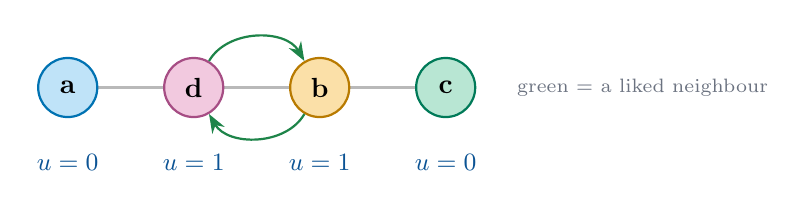
\begin{tikzpicture}
  \pathseat{a}{d}{b}{c}
  \draw[like] (d) to[out=60,in=120] (b);
  \draw[like] (b) to[out=-120,in=-60] (d);
  \foreach \x/\u in {0/0,1.6/1,3.2/1,4.8/0}{\node[ut] at (\x,-0.95) {$u=\u$};}
  \node[lab] at (7.3,0) {green = a liked neighbour};
\end{tikzpicture}
\end{center}
\begin{itemize}
  \item $a$ likes only $c$, who is far away: $u_a=0$. \; $d$ likes $b$ next to it: $u_d=1$.
\end{itemize}
\idea{An additively separable hedonic game with 0/1 values, where your ``group'' is your seat neighbourhood.}
\note{\tm{Ashik}{1:00}{5:15}
Formally, an agent's utility is the number of neighbours it likes. Nothing else counts.

Take the seating $a, d, b, c$ in a row. $a$ only likes $c$, who is at the other end, so $a$ gets 0. $d$ sits next to $b$, whom it likes: 1. $b$ also likes $d$: 1. $c$ likes only $a$: 0.

Course connection: we saw hedonic games where agents' value for a coalition is the sum of values for its members, i.e.\ additively separable. Here the values are 0 or 1. The difference is that the ``group'' you care about is not a coalition in a partition, but whoever ends up next to you on the seat graph. The paper itself points out this connection to hedonic games.}
\end{frame}

% ---------------------------------------------------------------- 6
\begin{frame}{Swaps, envy and blocking pairs}
\begin{itemize}
  \item $\pi^{i\leftrightarrow j}$: $\pi$ with $i$ and $j$ exchanging seats.
  \item $i$ \textbf{envies} $j$ if $u_i(\pi^{i\leftrightarrow j}) > u_i(\pi)$.
  \item $i,j$ form a \textbf{blocking pair} if each envies the other.
\end{itemize}
\vspace{1mm}
\begin{center}
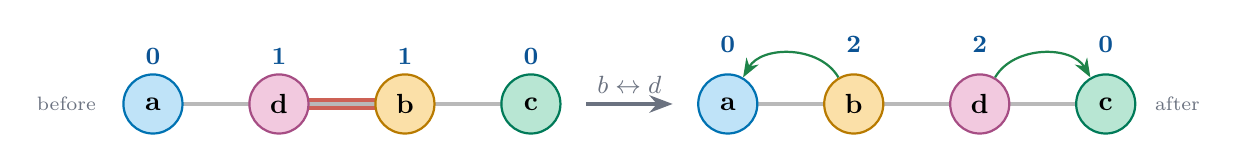
\begin{tikzpicture}
  \begin{scope}
    \draw[hot] (1.6,0)--(3.2,0);
    \pathseat{a}{d}{b}{c}
    \foreach \x/\u in {0/0,1.6/1,3.2/1,4.8/0}{\node[ut] at (\x,0.6) {\u};}
    \node[lab,anchor=east] at (-0.6,0) {before};
  \end{scope}
  \draw[-{Stealth},very thick,muted] (5.5,0) -- (6.6,0) node[midway,above,font=\small] {$b\leftrightarrow d$};
  \begin{scope}[xshift=7.3cm]
    \pathseat{a}{b}{d}{c}
    \draw[like] (b) to[out=120,in=60] (a);
    \draw[like] (d) to[out=60,in=120] (c);
    \foreach \x/\u in {0/0,1.6/2,3.2/2,4.8/0}{\node[ut] at (\x,0.75) {\u};}
    \node[lab,anchor=west] at (5.3,0) {after};
  \end{scope}
\end{tikzpicture}
\end{center}
\begin{itemize}
  \item $d$ trades neighbour $a$ (not liked) for $c$ (liked): $1\to 2$.
  \item $b$ trades neighbour $c$ (not liked) for $a$ (liked): $1\to 2$.
  \item Both gain, so $b,d$ is a blocking pair.
\end{itemize}
\note{\tm{Ashik}{1:30}{6:45}
Now the swap. Write $\pi^{i\leftrightarrow j}$ for the seating where $i$ and $j$ exchange seats. $i$ envies $j$ if $i$ would be strictly happier in $j$'s seat. A blocking pair is a pair where the envy goes both ways, so both would agree to swap.

Back to $a, d, b, c$. Look at $b$ and $d$ in the middle. If they swap, they are still next to each other, but $d$ moves next to $c$, whom it likes, and $b$ moves next to $a$, whom it likes. Both go from 1 to 2. So $b,d$ is a blocking pair.

Notice the pattern: when two neighbours swap, each one just trades its \emph{other} neighbour for the partner's other neighbour. Achyuth will use exactly this ``trade one neighbour'' view later.

These numbers are the paper's Example 1.}
\end{frame}

% ---------------------------------------------------------------- 7
\begin{frame}{Neighbourhood stability}
\begin{block}{Definition (neighbourhood stable, NS)}
An assignment $\pi$ is \textbf{neighbourhood stable} if no blocking pair sits on \textbf{adjacent} seats.
\end{block}
\vspace{2mm}
Compare: $\pi$ is \textbf{stable} if there is no blocking pair at all.
\vspace{5mm}

\textbf{Why only neighbours?}
\begin{itemize}\setlength\itemsep{2mm}
  \item To swap, two guests must first talk and agree.
  \item At a table you only talk to the people beside you.
  \item Guests may not even know where everyone else is sitting.
\end{itemize}
\note{\tm{Ashik}{1:00}{7:45}
This is the paper's central concept. A seating is \emph{neighbourhood stable} (I'll say NS) if no blocking pair sits next to each other. The usual notion, simply ``stable'', forbids blocking pairs anywhere at the table.

Why is the restriction natural? A swap needs the two guests to agree, which means they must talk. And you can only talk to the people next to you, which are exactly the people who affect your happiness. The paper also argues that NS is natural when agents have limited information about the overall seating.

So our earlier seating $a,d,b,c$ is not NS: $b$ and $d$ are neighbours and form a blocking pair.}
\end{frame}

% ---------------------------------------------------------------- 8
\begin{frame}{How the notions relate}
\begin{columns}[c]
\column{0.5\textwidth}
\centering
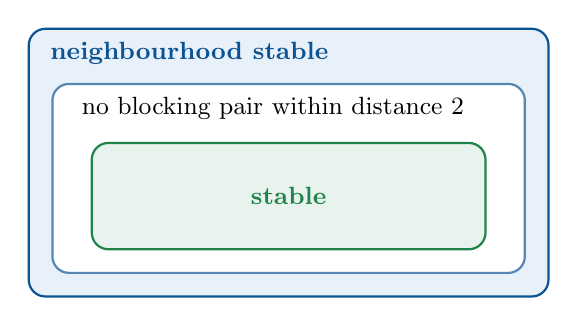
\begin{tikzpicture}
  \draw[rounded corners=6pt,thick,draw=accent,fill=linkbg] (0,0) rectangle (6.6,3.4);
  \node[anchor=north west,font=\small\bfseries,text=accent] at (0.15,3.35) {neighbourhood stable};
  \draw[rounded corners=6pt,thick,draw=accent!70,fill=white] (0.3,0.3) rectangle (6.3,2.7);
  \node[anchor=north west,font=\small] at (0.55,2.65) {no blocking pair within distance 2};
  \draw[rounded corners=6pt,thick,draw=good,fill=good!10] (0.8,0.6) rectangle (5.8,1.95);
  \node[font=\small\bfseries,text=good] at (3.3,1.28) {stable};
\end{tikzpicture}
\column{0.48\textwidth}
\begin{itemize}\setlength\itemsep{3mm}
  \item Running example after the swap, $a,b,d,c$: \textbf{stable}, hence also NS.
  \item NS is the weakest of the three, so it is the most likely to exist.
  \item Even checking whether a \emph{stable} seating exists is computationally hard.
\end{itemize}
\end{columns}
\note{\tm{Ashik}{0:30}{8:15}
The notions are nested. Stable means no blocking pair anywhere. In between, the earlier paper by Berriaud et al.\ looked at forbidding blocking pairs within distance two. NS only forbids distance one. So every stable seating is NS, but not the other way round.

For our running example, the seating after the swap, $a,b,d,c$, is in fact fully stable, so certainly NS. That is stated in the paper's Example 1.

Since NS is the weakest requirement, it has the best chance of always existing. The paper also notes that deciding existence of a fully stable seating is computationally hard, inherited from the exchange-stable roommates problem, which is NP-complete.}
\end{frame}

% ---------------------------------------------------------------- 9
\begin{frame}{Why binary (yes/no) preferences?}
Richer preferences already break NS on tiny instances:
\vspace{3mm}
\begin{itemize}\setlength\itemsep{3mm}
  \item \textbf{Three non-negative values}: 4 agents on a cycle with no NS assignment (from Berriaud et al.'s proof).
  \item \textbf{Values $\pm1$} (dislike allowed): fails already on a path of three seats.
  \item Two non-negative values are the same as binary, without loss of generality.
\end{itemize}
\vspace{5mm}
{\large So binary preferences are where positive results might live.}
\note{\tm{Ashik}{0:30}{8:45}
Why restrict to yes/no likes? Because anything richer fails almost immediately.

If an agent can value others at three levels, the paper points out, reusing a proof from Berriaud et al., that four agents on a cycle may have no NS seating. If dislikes are allowed, values plus or minus one, it fails even on a path of three seats. And two non-negative values reduce to binary.

So binary preferences are the natural setting to look for positive results, and the rest of the talk is about binary preferences.}
\end{frame}

% ---------------------------------------------------------------- 10
\begin{frame}{NS is genuinely weaker: two tables of three}
\begin{columns}[c]
\column{0.5\textwidth}
\centering
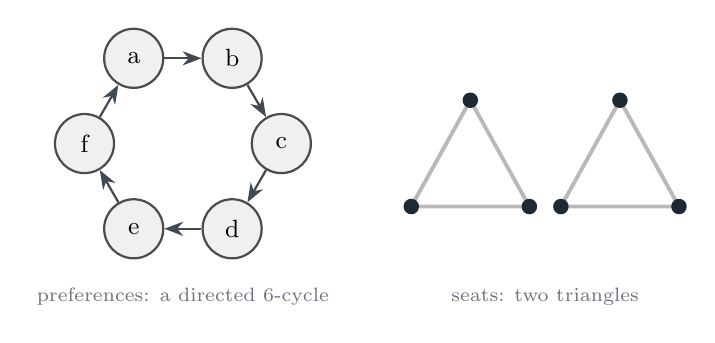
\begin{tikzpicture}
  \foreach \ang/\n in {120/a,60/b,0/c,-60/d,-120/e,180/f}{\node[agg] (\n) at (\ang:1.25) {\n};}
  \foreach \i/\j in {a/b,b/c,c/d,d/e,e/f,f/a}{\draw[arc] (\i)--(\j);}
  \node[lab] at (0,-1.95) {preferences: a directed 6-cycle};
  \begin{scope}[xshift=2.9cm,yshift=-0.8cm]
    \foreach \x in {0,1.9}{
      \draw[sedge] (\x,0)--(\x+1.5,0)--(\x+0.75,1.35)--cycle;
      \foreach \p in {(\x,0),(\x+1.5,0),(\x+0.75,1.35)}{\fill[ink] \p circle (2.8pt);}}
    \node[lab] at (1.7,-1.15) {seats: two triangles};
  \end{scope}
\end{tikzpicture}
\column{0.48\textwidth}
\begin{itemize}\setlength\itemsep{2mm}
  \item \textbf{No stable assignment:} some two agents at different tables both have utility 0, and they block.
  \item \textbf{Every assignment is NS:} neighbours share a table, and swapping them changes nobody's neighbours.
\end{itemize}
\vspace{2mm}
\src{Paper's Example 2, taken from Example 2 of Massand \& Simon, \emph{Graphical one-sided markets}, IJCAI 2019.}
\end{columns}
\note{\tm{Ashik}{1:30}{10:15}
Here is an example showing NS really is weaker than stability. Six agents, each likes exactly the next one around a directed 6-cycle. Seats: two separate tables of three, i.e.\ two triangles.

No stable seating exists: as the paper says, in every seating there are two agents at different tables who both have utility zero, and they would both gain by swapping, so they block. (Intuitively, a table of three can't contain everyone's single friend.)

But \emph{every} seating is NS. Neighbours are at the same table, and in a triangle, swapping two people leaves everyone with exactly the same neighbours. Nobody gains.

This example is taken from Massand and Simon, IJCAI 2019, \emph{Graphical one-sided markets}. Sunil Simon is our instructor.

We also brute-forced it: all 720 seatings are NS, none is stable.}
\end{frame}

% ---------------------------------------------------------------- 11
\begin{frame}{Theorem 1: NS assignments need not exist}
\begin{block}{Theorem 1}
For every $n=2t$ with $t\ge 3$ odd, there is an instance with $n$ agents and no NS assignment.
\end{block}
\begin{columns}[c]
\column{0.5\textwidth}
\centering
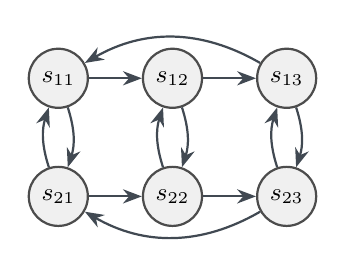
\begin{tikzpicture}[x=1.45cm,y=1.5cm]
  \foreach \j in {1,2,3}{
    \node[agg] (t\j) at (\j,1) {$s_{1\j}$};
    \node[agg] (b\j) at (\j,0) {$s_{2\j}$};
    \draw[arc] (t\j) to[bend left=18] (b\j); \draw[arc] (b\j) to[bend left=18] (t\j);}
  \draw[arc] (t1)--(t2); \draw[arc] (t2)--(t3); \draw[arc] (t3) to[bend right=30] (t1);
  \draw[arc] (b1)--(b2); \draw[arc] (b2)--(b3); \draw[arc] (b3) to[bend left=30] (b1);
\end{tikzpicture}\\
{\small each agent likes its \textbf{twin} and its \textbf{row successor}}
\column{0.45\textwidth}
\centering
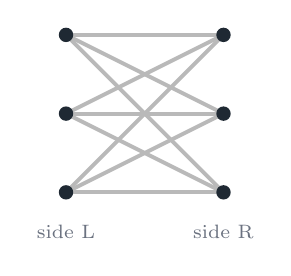
\begin{tikzpicture}
  \foreach \y in {0,1,2}{\foreach \z in {0,1,2}{\draw[sedge] (0,\y)--(2,\z);}}
  \foreach \y in {0,1,2}{\fill[ink] (0,\y) circle (2.6pt); \fill[ink] (2,\y) circle (2.6pt);}
  \node[lab] at (0,-0.5) {side L}; \node[lab] at (2,-0.5) {side R};
\end{tikzpicture}\\
{\small seat graph $K_{3,3}$ (complete bipartite)}
\end{columns}
\vspace{1mm}
\src{Paper's Fig.~1 ($t=3$). We also checked all $6!=720$ seatings: none is NS.}
\note{\tm{Ashik}{1:00}{11:15}
Now the bad news. Theorem 1: for every even $n = 2t$ with $t$ odd and at least 3, there's an instance with no NS seating at all.

The construction: seats form the complete bipartite graph $K_{t,t}$, two sides, every seat on one side next to every seat on the other side. Like two rows facing each other where everyone talks to everyone across.

Agents come in two rows, top $s_{1j}$ and bottom $s_{2j}$. Each agent likes exactly two people: its twin in the other row (the vertical 2-cycles), and its successor in its own row (the two directed $t$-cycles). Here $t=3$, which is the paper's Figure 1 with six agents.

We verified the six-agent case by brute force: none of the 720 seatings is NS.}
\end{frame}

% ---------------------------------------------------------------- 12
\begin{frame}{Theorem 1, key idea: only your side matters}
\begin{itemize}\setlength\itemsep{2mm}
  \item In $K_{t,t}$ your neighbours are \emph{everyone on the other side}. So a seating is just a split into sides $L$ and $R$.
  \item Everyone likes exactly 2 agents; utility = how many of them are across.
\end{itemize}
\vspace{2mm}
Two ways for $i$ to envy an agent $j$ across:
\begin{itemize}\setlength\itemsep{2mm}
  \item[\textbf{(C1)}] $i$ likes \textbf{both} its favourites on its own side ($u_i=0$). Then $i$ envies \emph{everyone} across: $0\to 2$.
  \item[\textbf{(C2)}] $i$ likes \textbf{one} agent on its own side and also likes $j$. Then $i$ envies $j$: $1\to 2$.
\end{itemize}
\note{\tm{Ashik}{1:15}{12:30}
Here is the trick that makes the proof manageable. In a complete bipartite seat graph, your neighbours are \emph{all} the people on the opposite side. So the only thing that matters is which side each agent is on.

Each agent likes exactly two others, so utility is 0, 1 or 2: the number of its two favourites who are across.

If $i$ swaps with some $j$ across, $i$ moves to the other side; its new neighbours are its old side-mates plus $j$. That gives two simple envy conditions.

C1: if both of $i$'s favourites are on $i$'s own side, $i$ has 0 and would get 2 by moving across: $i$ envies everyone across.

C2: if one favourite is on $i$'s side and the other favourite is $j$ across, then swapping with $j$ gives 2 instead of 1.

The proof shows that in every split, some pair envy each other this way. Since they're on opposite sides, they're adjacent.}
\end{frame}

% ---------------------------------------------------------------- 13
\begin{frame}{Theorem 1, proof sketch: a blocking pair always appears}
\begin{columns}[T]
\column{0.48\textwidth}
\textbf{\color{accent}Case 1: some twins sit together}
\begin{itemize}\setlength\itemsep{2mm}
  \item $t$ odd $\Rightarrow$ some other twin pair is split.
  \item Some agent then has $u=0$ and envies the whole other side (C1).
  \item Following the twins around the row finds an agent that envies it back (C2).
\end{itemize}
\column{0.48\textwidth}
\textbf{\color{accent}Case 2: all twins split}
\begin{itemize}\setlength\itemsep{2mm}
  \item $t$ odd $\Rightarrow$ two \emph{consecutive} agents of one row share a side.
  \item One of them and its twin envy each other (C2).
\end{itemize}
\end{columns}
\idea{Both cases use that $t$ is odd.}
\note{\tm{Ashik}{1:45}{14:15}
Two cases, depending on whether some twins sit on the same side.

Case 2 is the cleaner one; start there. Suppose every twin pair is split. Then each side holds exactly one of each pair, so at least $\lceil t/2\rceil$ agents on one side come from the same row, say the top. They lie on a directed $t$-cycle; an odd cycle has no independent set larger than $\lfloor t/2\rfloor$, so two consecutive top agents $s_{1j}, s_{1,j+1}$ are on the same side. Then $s_{1j}$ likes $s_{1,j+1}$ on its side and likes its twin across: C2, it envies its twin. Symmetrically the twin $s_{2j}$ likes its successor (which is across from $s_{1,j+1}$, on its own side) and likes $s_{1j}$: C2. Blocking pair.

Case 1: some twins are together. Parity forces some split twin, so we can find $j$ where twins $j$ are together and twins $j+1$ are split. That $s_{1j}$ has both favourites on its side: utility 0, envies everyone across. To avoid an immediate blocking pair, nobody across may have 0. That forces a pattern: every together-pair on the right is followed by a together-pair on the left. Counting, the pair just before $j$ must be together on the right, and its top agent envies $s_{1j}$ by C2. Blocking pair.

Main message: oddness is used in both cases.}
\end{frame}

% ---------------------------------------------------------------- 14
\begin{frame}{Proposition 1: letting guests swap can loop forever}
\begin{columns}[c]
\column{0.2\textwidth}
\centering
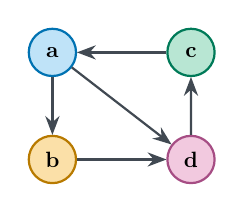
\begin{tikzpicture}[scale=0.8,every node/.style={transform shape}]\figsixpref\end{tikzpicture}\\[1mm]
{\scriptsize preferences (Fig.~6)}
\column{0.8\textwidth}
\centering
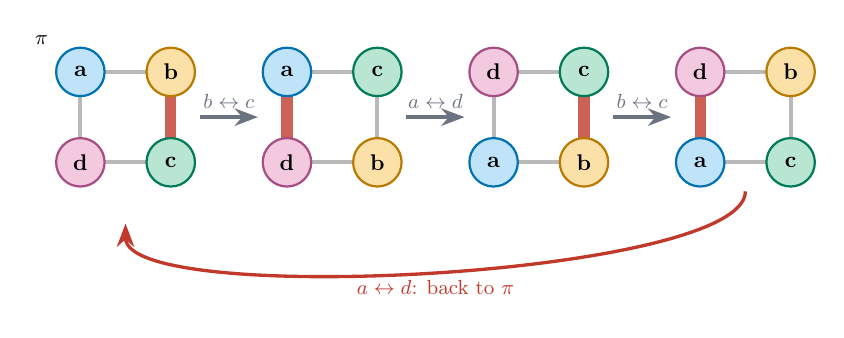
\begin{tikzpicture}[scale=0.82,every node/.style={transform shape}]
  \begin{scope}[xshift=0cm]\sqseat{a}{b}{c}{d}{b}{c}\node[font=\small\bfseries] at (-0.6,1.9) {$\pi$};\end{scope}
  \begin{scope}[xshift=3.2cm]\sqseat{a}{c}{b}{d}{a}{d}\end{scope}
  \begin{scope}[xshift=6.4cm]\sqseat{d}{c}{b}{a}{c}{b}\end{scope}
  \begin{scope}[xshift=9.6cm]\sqseat{d}{b}{c}{a}{d}{a}\end{scope}
  \foreach \x/\l in {1.85/{b\leftrightarrow c},5.05/{a\leftrightarrow d},8.25/{b\leftrightarrow c}}{
    \draw[-{Stealth},very thick,muted] (\x,0.7)--(\x+0.9,0.7) node[midway,above,font=\small] {$\l$};}
  \draw[-{Stealth},very thick,warn] (10.3,-0.45) to[out=-90,in=-90,looseness=0.35] node[below,font=\small] {$a\leftrightarrow d$: back to $\pi$} (0.7,-0.95);
\end{tikzpicture}
\end{columns}
\vspace{2mm}
\begin{itemize}\setlength\itemsep{2mm}
  \item Red = the \textbf{only} blocking pair in that seating; both swappers gain.
  \item Swapping blocking neighbours can \textbf{cycle forever}, even on 4 seats.
\end{itemize}
\note{\tm{Ashik}{1:45}{16:00}
A natural idea: start anywhere and let neighbours who form a blocking pair swap, until nobody wants to. The paper calls this swap dynamics. Proposition 1 says this can fail even on a round table with four seats.

Different preferences here (the paper's Fig.~6, left): $c$ likes $a$; $a$ likes $b$ and $d$; $b$ likes $d$; $d$ likes $c$.

Start with $a,b,c,d$ around the square. $b$ and $c$ have 0 each; if they swap, each gets 1. Swap. Now $a$ and $d$ block: $a$ goes from 1 to 2, $d$ from 0 to 1. Swap. Then $b,c$ again, then $a,d$ again, and we're back where we started.

Crucially, the paper checks that the highlighted pair is the \emph{unique} blocking pair at every step. So it's not bad luck in choosing which pair swaps; there is no other choice. (Our script confirms the loop and the uniqueness.)}
\end{frame}

% ---------------------------------------------------------------- 15
\begin{frame}{What Proposition 1 tells us}
\begin{itemize}\setlength\itemsep{4mm}
  \item An \textbf{improvement cycle}: no potential can rise with every swap.
  \item From this start, \emph{every} sequence of swaps loops.
  \item Yet NS seatings do exist here.
\end{itemize}
\vspace{2mm}
\idea{No finite improvement property (FIP), not even weakly acyclic.\\ So on cycles we need an \textbf{algorithm}, not dynamics.}
\note{\tm{Ashik}{1:00}{17:00}
Let me connect this to what we did in class.

A loop of strictly improving moves is an improvement cycle. In potential games, the finite improvement property, FIP, is equivalent to having a generalised ordinal potential. So, by analogy, there can be no potential function for swap dynamics on cycles. In fact it's worse: because each blocking pair is unique, from this start \emph{no} sequence of swaps ever terminates. So it's not even weakly acyclic, unlike the colouring games we saw.

But the instance does have NS seatings (the paper says so; we counted 8 of the 24). So for cycles we need a constructive argument, not dynamics.

Contrast, for when swaps do work: the paper remarks that symmetric preferences guarantee NS. Our own quick argument: when likes are mutual, a blocking swap increases the number of adjacent mutually-liking pairs by exactly the two swappers' total gain, so it's a potential.

Handover: Achyuth will now show how to construct NS seatings.}
\end{frame}

% =====================================================================
\def\who{}
% ---------------------------------------------------------------- 16
\begin{frame}{Map of results}
\renewcommand{\arraystretch}{1.35}
\begin{center}
\begin{tabular}{@{}lll@{}}
\toprule
\textbf{Seat graph} & \textbf{Guarantee} & \textbf{Algorithm} \\
\midrule
$K_{t,t}$, $t\ge3$ odd & {\color{warn}NS may not exist} (Thm 1) & -- \\
Cycle & {\color{good}NS always exists} (Thm 2) & $O(n^3)$ \\
Path & {\color{good}no blocking pair within distance 2} (Thm 3) & $O(n^2)$ \\
Enough leaves & {\color{good}NS exists} (Thm 4) & poly.\ if $\mathcal{P}$ is a DAG \\
\bottomrule
\end{tabular}
\end{center}
\vspace{4mm}
\small DFVS = directed feedback vertex set (explained with Theorem 4); DAG = directed acyclic graph.\\
$O(n^2)$, $O(n^3)$: running time grows at most like the square / cube of the number of agents.
\note{\tm{Achyuth}{1:00}{18:00}
Thanks, Ashik. Here's the map of what the paper proves.

Ashik showed the negative result on complete bipartite seat graphs. The positive results are:
\begin{itemize}
\item On a cycle, a round table, an NS seating always exists, computed in cubic time. This is the central result and I'll spend most time on it.
\item On a path, a bench, something even stronger: no blocking pair within distance two, also cubic time.
\item On any seat graph, if it has enough leaves, measured against how far the preference graph is from acyclic, NS exists; and when the preferences have no cycles at all, it's computable in polynomial time.
\end{itemize}}
\end{frame}

% ---------------------------------------------------------------- 17
\begin{frame}{Theorem 2: round tables always work}
\begin{block}{Theorem 2 (central result)}
If the seat graph is a cycle, an NS assignment always exists and can be computed in $O(n^3)$ time.
\end{block}
\vspace{3mm}
Why this is surprising:
\begin{itemize}\setlength\itemsep{2mm}
  \item Forbidding blocking pairs within distance 2 can fail on a 5-agent cycle (Berriaud et al.).
  \item With 3-valued preferences it fails on a 4-agent cycle.
  \item Swap dynamics can loop (Proposition 1).
\end{itemize}
\note{\tm{Achyuth}{0:30}{18:30}
Theorem 2: on a cycle, an NS seating always exists, and we can find one in $O(n^3)$ time.

The paper calls this surprising, and here's why. Berriaud et al.\ showed that if you also forbid blocking pairs at distance two, it can fail with just five agents on a cycle. With three-valued preferences it fails on four agents. And as Ashik showed, the swap dynamics can loop. Yet with binary preferences and only adjacent swaps, it always works.}
\end{frame}

% ---------------------------------------------------------------- 18
\begin{frame}{The one tool we need: a swap trades one neighbour}
\begin{center}
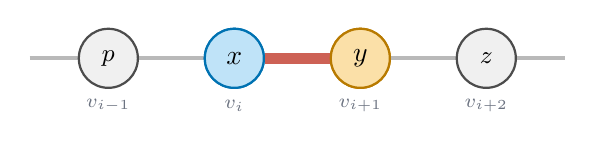
\begin{tikzpicture}
  \draw[sedge] (-1,0)--(5.8,0);
  \node[agg] (p) at (0,0) {$p$}; \node[aga] (x) at (1.6,0) {$x$};
  \node[agb] (y) at (3.2,0) {$y$}; \node[agg] (z) at (4.8,0) {$z$};
  \foreach \x/\v in {0/{i-1},1.6/{i},3.2/{i+1},4.8/{i+2}}{\node[lab] at (\x,-0.6) {$v_{\v}$};}
  \draw[hot] (x)--(y); \node[aga] at (1.6,0) {$x$}; \node[agb] at (3.2,0) {$y$};
\end{tikzpicture}
\end{center}
When neighbours $x,y$ swap on a cycle, they stay adjacent. So:
\begin{itemize}
  \item $x$ gives up $p$ and gets $z$; \quad $y$ gives up $z$ and gets $p$.
\end{itemize}
\vspace{1mm}
\begin{center}
\colorbox{linkbg}{\parbox{0.86\textwidth}{\centering
$x,y$ block \quad$\iff$\quad $x\to z,\ \ x\nlikes p$ \quad and \quad $y\to p,\ \ y\nlikes z$}}
\end{center}
\vspace{1mm}
\small
\begin{itemize}
  \item \textbf{Obs.~2:} if $x$ already likes $p$, then $x$ will not envy $y$.
  \item \textbf{Obs.~1:} if $y\nlikes p$ or $x\nlikes z$, then $x,y$ cannot block.
\end{itemize}
\note{\tm{Achyuth}{1:30}{20:00}
Everything on cycles rests on one simple observation, which Ashik hinted at.

Take two neighbours $x$ and $y$ on the cycle, with $p$ on $x$'s other side and $z$ on $y$'s other side. If $x$ and $y$ swap, they're still next to each other. The only change for $x$ is that it loses $p$ and gains $z$. For $y$, it loses $z$ and gains $p$.

So $x$ envies $y$ exactly when $x$ likes $z$ but not $p$. And $y$ envies $x$ exactly when $y$ likes $p$ but not $z$. A blocking pair needs all four conditions.

The paper states this as two observations. Observation 2: if you already like the neighbour you'd lose, you won't envy. Observation 1: if $y$ doesn't like $p$, or $x$ doesn't like $z$, no blocking pair.

Check with Ashik's example: $d$ was $x$, $b$ was $y$, $p=a$, $z=c$. $d$ likes $c$ not $a$; $b$ likes $a$ not $c$. All four hold: blocking.}
\end{frame}

% ---------------------------------------------------------------- 19
\begin{frame}{Two cases, depending on the preference graph}
\begin{columns}[T]
\column{0.48\textwidth}
\textbf{\color{accent}Case 1: there is a ``V''}\\[2mm]
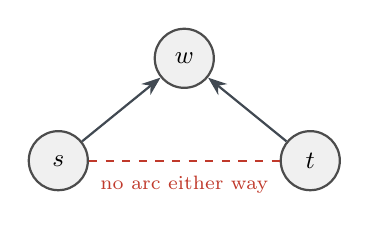
\begin{tikzpicture}
  \node[agg] (s) at (0,0) {$s$}; \node[agg] (w) at (1.6,1.3) {$w$}; \node[agg] (t) at (3.2,0) {$t$};
  \draw[arc] (s)--(w); \draw[arc] (t)--(w);
  \draw[dashed,warn,thick] (s)--(t) node[midway,below=2pt,font=\scriptsize,text=warn] {no arc either way};
\end{tikzpicture}\\[2mm]
\small Two agents like the same $w$ but neither likes the other.\\[2mm]
Running example: $b\to a\leftarrow c$, and $b,c$ unrelated.
\column{0.48\textwidth}
\textbf{\color{accent}Case 2: no ``V''}\\[2mm]
\small Whenever two agents like the same person, one of them likes the other.\\[3mm]
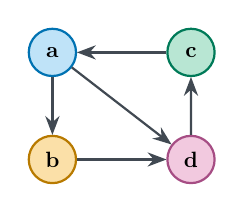
\begin{tikzpicture}[scale=0.8,every node/.style={transform shape}]\figsixpref\end{tikzpicture}\\[1mm]
The looping instance (Fig.~6) is in Case 2: only $d$ has two admirers, $a$ and $b$, and $a\to b$.
\end{columns}
\vspace{2mm}
\small Testing every triple of agents decides the case in $O(n^3)$ time.
\note{\tm{Achyuth}{1:00}{21:00}
Algorithm 1 splits into two cases based only on the preference graph.

Case 1: there's a ``V''. Two agents $s$ and $t$ both like the same $w$, but there's no arrow between $s$ and $t$ in either direction. Our running example has one: $b$ and $c$ both like $a$, and $b$, $c$ are unrelated.

Case 2: no V. Whenever two people like the same person, one of them likes the other. Ashik's looping example falls here: only $d$ has two admirers, $a$ and $b$, and $a$ likes $b$.

Checking which case we're in just means looking at all triples: cubic time.}
\end{frame}

% ---------------------------------------------------------------- 20
\begin{frame}{Case 1: a greedy seating}
\begin{columns}[c]
\column{0.55\textwidth}
\textbf{Algorithm (Case 1)}
\begin{enumerate}\setlength\itemsep{2mm}
  \item Seat $s, w, t$ on $v_1, v_2, v_3$.
  \item For $v_4, v_5, \dots, v_n$: seat an unseated agent who \textbf{likes the previous seat's agent}; if there is none, seat anyone.
\end{enumerate}
\vspace{3mm}
\textbf{Run on the running example:}\\
$s=b,\ w=a,\ t=c$. \ Only $d$ is left, and $d$ likes $c$, so $d$ takes $v_4$.
\column{0.42\textwidth}
\centering
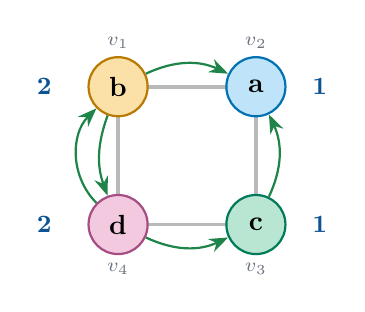
\begin{tikzpicture}[scale=1.25]
  \sqseat{b}{a}{c}{d}{b}{b}
  \draw[like] (b) to[bend left=25] (a);
  \draw[like] (c) to[bend right=25] (a);
  \draw[like] (d) to[bend right=25] (c);
  \draw[like] (b) to[bend right=20] (d);
  \draw[like] (d) to[bend left=45] (b);
  \node[lab] at (0,1.85) {$v_1$}; \node[lab] at (1.4,1.85) {$v_2$};
  \node[lab] at (1.4,-0.45) {$v_3$}; \node[lab] at (0,-0.45) {$v_4$};
  \node[ut] at (-0.75,1.4) {2}; \node[ut] at (2.05,1.4) {1};
  \node[ut] at (2.05,0) {1}; \node[ut] at (-0.75,0) {2};
\end{tikzpicture}\\
{\small Everyone gets their maximum possible utility.}
\end{columns}
\note{\tm{Achyuth}{1:30}{22:30}
Case 1 is solved by a simple greedy rule.

Put the V on the first three seats: $s$, then $w$, then $t$. Then go round the table: for each next seat, pick an unseated agent who likes the agent in the previous seat, if possible; otherwise anyone.

On our running example: $s=b$, $w=a$, $t=c$. For seat 4 we need an unseated agent who likes $c$. Only $d$ is left, and $d$ does like $c$. So the table is $b, a, c, d$.

Utilities: $b$ sits between $a$ and $d$, likes both: 2. $a$ is next to $c$: 1, and $a$ only likes $c$, so that's its max. Same for $c$. $d$ is next to $b$ and $c$: 2. Everyone is at their maximum, so clearly NS. We verified this in code too.

Note on this picture: green arrows are likes between neighbours.}
\end{frame}

% ---------------------------------------------------------------- 21
\begin{frame}{Why the greedy seating is NS}
Recall: $x,y$ (with $p$ left of $x$) block only if $y\to p$ and $x\nlikes p$.
\vspace{3mm}
\begin{itemize}\setlength\itemsep{3mm}
  \item \textbf{Around the V:} $s\nlikes t$, so $s$ won't envy $w$; \ $t\nlikes s$, so $t$ won't envy $w$.\\
        $s$ and $t$ both like $w$, so neither envies its other neighbour.
  \item \textbf{Everywhere else:} take neighbours $x$ (at $v_i$) and $y$ (at $v_{i+1}$).
  \begin{itemize}
    \item If $x\to p$: no envy from $x$ (Obs.~2).
    \item If $x\nlikes p$: when $x$ was chosen, \emph{nobody} unseated liked $p$, including $y$. So $y\nlikes p$ (Obs.~1).
  \end{itemize}
\end{itemize}
\vspace{3mm}
\colorbox{linkbg}{\parbox{0.95\linewidth}{\small \textbf{Invariant:} for every pair $x,y$, either $x$ likes the agent on its left, or $y$ does not. That is all NS needs.}}
\note{\tm{Achyuth}{1:15}{23:45}
Why does this work? Use the swap rule: $x$ and $y$ block only if $y$ likes $p$ while $x$ doesn't.

Around the V it's by design: $s$ doesn't like $t$, so swapping with $w$ (gaining $t$) is useless for $s$. Likewise $t$ doesn't like $s$. And $s$, $t$ both like $w$, so they won't give $w$ up by swapping with their other neighbours.

Everywhere else, the greedy invariant does the job. When we chose $x$ for seat $v_i$, we picked someone who likes $p$ if anyone could. If $x$ does not like $p$, then nobody unseated liked $p$ at that time, and $y$ was unseated then. So $y$ doesn't like $p$ either, and $y$ has no reason to swap. Either way, no blocking pair.

The V is needed to start the cycle safely: the first and last seats wrap around.}
\end{frame}

% ---------------------------------------------------------------- 22
\begin{frame}{Case 2: wrap path partitions around the table}
\begin{columns}[c]
\column{0.42\textwidth}
\centering
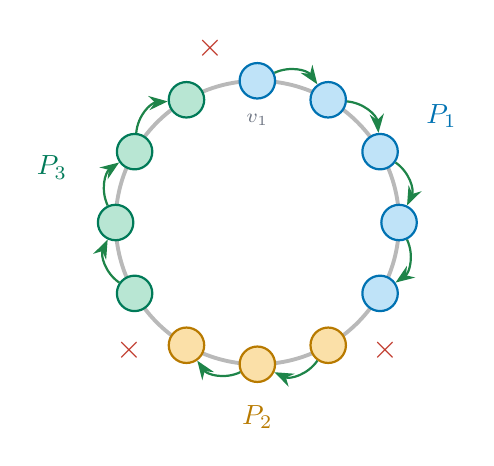
\begin{tikzpicture}[scale=0.9]
  \draw[sedge] (0,0) circle (2);
  \foreach \k/\st in {0/aga,1/aga,2/aga,3/aga,4/aga,5/agb,6/agb,7/agb,8/agc,9/agc,10/agc,11/agc}{
    \node[\st,minimum size=4.5mm] (s\k) at ({90-30*\k}:2) {};}
  \foreach \k in {0,1,2,3,5,6,8,9,10}{\pgfmathtruncatemacro\nx{\k+1}\draw[like] (s\k) to[bend left=40] (s\nx);}
  \foreach \k in {4,7,11}{\node[text=warn,font=\large\bfseries] at ({90-30*(\k+0.5)}:2.55) {$\times$};}
  \node[font=\bfseries,text=Adraw] at (30:3.0) {$P_1$};
  \node[font=\bfseries,text=Bdraw] at (-90:2.75) {$P_2$};
  \node[font=\bfseries,text=Cdraw] at (165:3.0) {$P_3$};
  \node[lab] at (90:1.45) {$v_1$};
\end{tikzpicture}
\column{0.56\textwidth}
\begin{itemize}\setlength\itemsep{2mm}
  \item \textbf{Path partition:} split the agents into directed paths (each agent likes the next one).
  \item \textbf{$\Phi(P_1,\dots,P_k)$:} lay the paths around the cycle, one after another.
  \item \textbf{Minimal:} no path's tail likes another path's head (otherwise glue them).
  \item \textbf{Start:} repeatedly remove a maximal path. This gives a minimal partition.
\end{itemize}
\vspace{1mm}
\small \textbf{Progress:} $R$ = number of agents who like their right neighbour.
\end{columns}
\note{\tm{Achyuth}{1:30}{25:30}
Case 2 is the interesting one, and it's the paper's new technique: path partitions.

Split all agents into directed paths in the preference graph: each agent on a path likes the next one. Then lay these paths around the table one after another; the paper calls this seating $\Phi$. This picture is like the paper's Figure 4. Inside a path, everyone likes their right-hand neighbour (green arrows). The red crosses are the boundaries, where a path's tail sits next to the next path's head.

A partition is minimal if no tail likes another path's head. If one did, we'd just glue the two paths together. To start, take a maximal path, remove it, repeat; that is automatically minimal.

Keep in mind the progress measure: the number of agents who like their right-hand neighbour. Fewer paths means more of these. The algorithm will strictly increase this number.}
\end{frame}

% ---------------------------------------------------------------- 23
\begin{frame}{Claim 1: in Case 2 you can always squeeze in}
\begin{center}
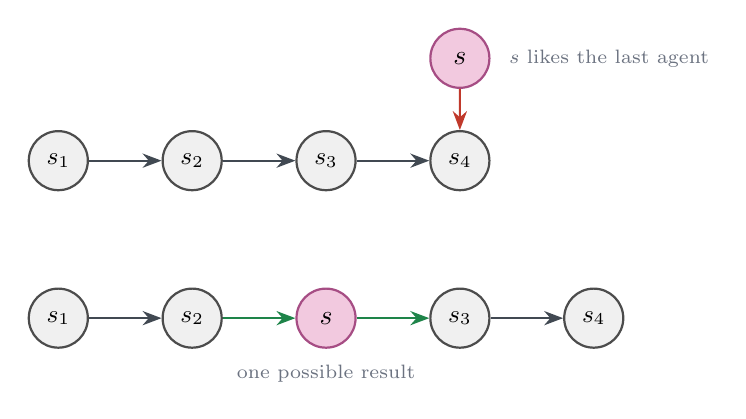
\begin{tikzpicture}
  \foreach \i in {1,...,4}{\node[agg] (s\i) at ({(\i-1)*1.7},0) {$s_\i$};}
  \foreach \i/\j in {1/2,2/3,3/4}{\draw[arc] (s\i)--(s\j);}
  \node[agd] (s) at (5.1,1.3) {$s$};
  \draw[bad] (s)--(s4);
  \node[lab,anchor=west] at (5.6,1.3) {$s$ likes the last agent};
  \begin{scope}[yshift=-2cm]
    \node[agg] (u1) at (0,0) {$s_1$}; \node[agg] (u2) at (1.7,0) {$s_2$};
    \node[agd] (us) at (3.4,0) {$s$};
    \node[agg] (u3) at (5.1,0) {$s_3$}; \node[agg] (u4) at (6.8,0) {$s_4$};
    \draw[arc] (u1)--(u2); \draw[like] (u2)--(us); \draw[like] (us)--(u3); \draw[arc] (u3)--(u4);
    \node[lab] at (3.4,-0.7) {one possible result};
  \end{scope}
\end{tikzpicture}
\end{center}
\textbf{Claim 1.} If $s$ likes the last agent of a path, $s$ can be inserted into the path.\\[2mm]
\textbf{Why:} $s$ and $s_3$ both like $s_4$, so one likes the other (no V). Insert, or step back and repeat.
\note{\tm{Achyuth}{0:45}{26:00}
One helper fact for Case 2. Suppose an outsider $s$ likes the last agent of a path. Then $s$ can be inserted somewhere into the path while keeping it a path.

Why? $s$ and $s_{r-1}$ both like $s_r$. In Case 2 there's no V, so one of them likes the other. If $s_{r-1}$ likes $s$, insert $s$ right there: $s_{r-1}\to s\to s_r$. Otherwise $s$ likes $s_{r-1}$, and we repeat the argument one step back. Eventually we either insert or reach the front, and $s$ likes $s_1$ so we prepend. Formally it's an induction on the path length.

Note this is exactly where Case 2's ``no V'' property gets used.}
\end{frame}

% ---------------------------------------------------------------- 24
\begin{frame}{Lemma 1: repairing a blocking pair merges two paths}
\begin{center}
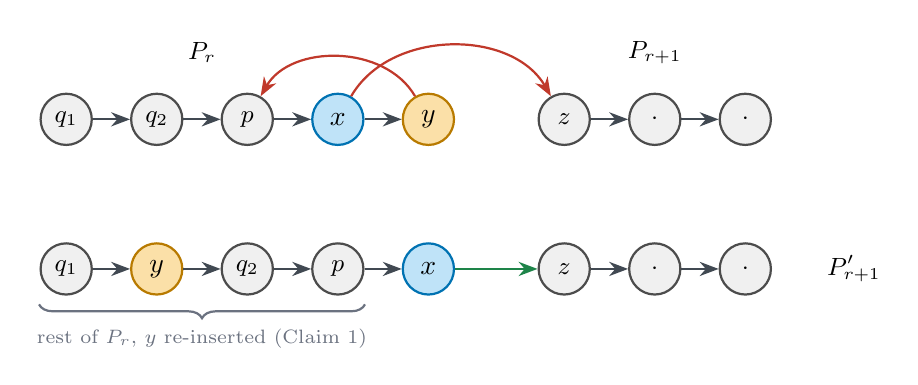
\begin{tikzpicture}[x=1.15cm]
  \node[agg,minimum size=6.5mm] (q1) at (0,1.9) {$q_1$}; \node[agg,minimum size=6.5mm] (q2) at (1,1.9) {$q_2$};
  \node[agg,minimum size=6.5mm] (p) at (2,1.9) {$p$}; \node[aga,minimum size=6.5mm] (x) at (3,1.9) {$x$};
  \node[agb,minimum size=6.5mm] (y) at (4,1.9) {$y$}; \node[agg,minimum size=6.5mm] (z) at (5.5,1.9) {$z$};
  \node[agg,minimum size=6.5mm] (z2) at (6.5,1.9) {$\cdot$}; \node[agg,minimum size=6.5mm] (z3) at (7.5,1.9) {$\cdot$};
  \draw[arc] (q1)--(q2); \draw[arc] (q2)--(p); \draw[arc] (p)--(x); \draw[arc] (x)--(y);
  \draw[arc] (z)--(z2); \draw[arc] (z2)--(z3);
  \draw[bad] (y) to[out=120,in=60] (p);
  \draw[bad] (x) to[out=60,in=120] (z);
  \node[font=\small\bfseries] at (1.5,2.75) {$P_r$}; \node[font=\small\bfseries] at (6.5,2.75) {$P_{r+1}$};
  \node[agg,minimum size=6.5mm] (b1) at (0,0) {$q_1$}; \node[agb,minimum size=6.5mm] (b2) at (1,0) {$y$};
  \node[agg,minimum size=6.5mm] (b3) at (2,0) {$q_2$}; \node[agg,minimum size=6.5mm] (b4) at (3,0) {$p$};
  \node[aga,minimum size=6.5mm] (b5) at (4,0) {$x$}; \node[agg,minimum size=6.5mm] (b6) at (5.5,0) {$z$};
  \node[agg,minimum size=6.5mm] (b7) at (6.5,0) {$\cdot$}; \node[agg,minimum size=6.5mm] (b8) at (7.5,0) {$\cdot$};
  \draw[arc] (b1)--(b2); \draw[arc] (b2)--(b3); \draw[arc] (b3)--(b4); \draw[arc] (b4)--(b5);
  \draw[like] (b5)--(b6); \draw[arc] (b6)--(b7); \draw[arc] (b7)--(b8);
  \draw[decorate,decoration={brace,mirror,amplitude=5pt},thick,muted] (-0.3,-0.45)--(3.3,-0.45) node[midway,below=5pt,font=\scriptsize] {rest of $P_r$, $y$ re-inserted (Claim 1)};
  \node[font=\small\bfseries] at (8.7,0) {$P'_{r+1}$};
\end{tikzpicture}
\end{center}
\textbf{Case: $x,y$ in the same path.}
\begin{itemize}
  \item Blocking forces $y$ = tail, $z$ = next head, and $y\to p$, $x\to z$ (red).
  \item Re-insert $y$ (Claim 1), then glue $p\to x\to z$: \textbf{one fewer path}.
\end{itemize}
\note{\tm{Achyuth}{2:00}{28:00}
This is the heart of the cycle proof. Suppose the seating from our path partition has a blocking pair $x,y$. Lemma 1 says we can build a new minimal partition with fewer paths.

Type I: $x$ and $y$ are consecutive in the same path. By the swap rule, $y$ must not like $z$, its right neighbour. Inside a path everyone likes the next one, so $y$ must be the \emph{tail} of its path and $z$ the head of the next path. The swap rule also says $y$ likes $p$ and $x$ likes $z$: those are the two red arrows.

Repair, as in the paper's Figure 5: remove $x$ and $y$ from the end of $P_r$. The remaining path ends at $p$, and $y$ likes $p$, so by Claim 1 we can re-insert $y$ somewhere. The path still ends at $p$; $p$ likes $x$; and $x$ likes $z$. So we can glue everything onto $P_{r+1}$. Two paths became one.

If $P_r$ has only two agents, it's similar: $y$ goes into the previous path and $x$ goes in front of the next one.

Then make it minimal again by gluing whatever can be glued. Fewer paths means more agents liking their right-hand neighbour.}
\end{frame}

% ---------------------------------------------------------------- 25
\begin{frame}{Finishing Theorem 2}
\begin{columns}[c]
\column{0.6\textwidth}
\begin{itemize}\setlength\itemsep{3mm}
  \item A blocking pair cannot straddle two paths: that would contradict minimality.
  \item $R\le n$ and each repair raises $R$: at most $n$ repairs, $O(n^3)$ total.
  \item Fig.~6: the path $c\to a\to b\to d$, wrapped around, is NS at once.
\end{itemize}
\idea{A progress measure, as for Hopfield networks, but with only $n{+}1$ values: no exponential search as in PLS (Polynomial Local Search).}
\column{0.36\textwidth}
\centering
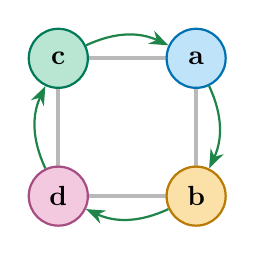
\begin{tikzpicture}[scale=1.25]
  \sqseat{c}{a}{b}{d}{c}{c}
  \draw[like] (c) to[bend left=25] (a); \draw[like] (a) to[bend left=25] (b);
  \draw[like] (b) to[bend left=25] (d); \draw[like] (d) to[bend left=25] (c);
\end{tikzpicture}\\[1mm]
{\scriptsize Fig.~6 instance, path $c\to a\to b\to d$\\(swap dynamics looped here)}
\end{columns}
\note{\tm{Achyuth}{1:30}{29:30}
The other type of blocking pair straddles a boundary: $x$ is the tail of one path, $y$ the head of the next. The swap rule needs $y$ not to like $z$. But if $y$'s path had a second agent, $y$ would like it. So $y$ is alone, and $z$ is the head of the path after that. And $x$ must like $z$: a tail liking another head, contradicting minimality. So Type II can't happen.

Termination: the number of agents who like their right neighbour is at most $n$, and each repair raises it. So at most $n$ repairs, each quadratic, cubic overall.

On Ashik's looping instance, if the algorithm's maximal path is $c\to a\to b\to d$, it covers everyone, $d$ likes $c$, and wrapping it round the table is already NS.

Course link: this is a progress-measure argument like the energy in Hopfield networks, but the measure has at most $n+1$ values, so no exponential PLS-style search. Note the moves here are the algorithm's re-arrangements, not guests' swaps.}
\end{frame}

% ---------------------------------------------------------------- 26
\begin{frame}{Theorem 3: benches (paths)}
\begin{block}{Theorem 3}
If the seat graph is a path, an assignment with \textbf{no blocking pair within distance 2} exists and is computed in $O(n^2)$ time.
\end{block}
\begin{columns}[c]
\column{0.5\textwidth}
\textbf{Same greedy:} each next seat gets someone who likes the previous agent.\\[2mm]
Running example: $a$, $c$, $d$, $b$.
\column{0.48\textwidth}
\centering
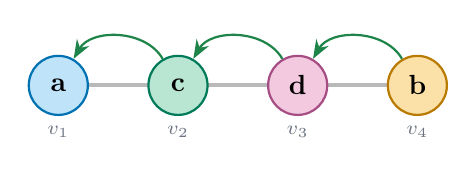
\begin{tikzpicture}[scale=0.95]
  \pathseat{a}{c}{d}{b}
  \draw[like] (c) to[out=120,in=60] (a);
  \draw[like] (d) to[out=120,in=60] (c);
  \draw[like] (b) to[out=120,in=60] (d);
  \seatlabels
\end{tikzpicture}\\
{\scriptsize fully stable (checked by brute force)}
\end{columns}
\idea{Swapping also converges on paths (Berriaud et al.), but maybe exponentially slowly.\\ This paper settles their open question with a direct, fast construction.}
\note{\tm{Achyuth}{1:30}{31:00}
For a bench, a path seat graph, the paper gets something stronger than NS: no blocking pair within distance two. Running time: each of the $n$ seats needs one scan of the unseated agents, so $O(n^2)$. (If asked: the paper's theorem states $O(n^3)$, which is a looser bound; the greedy itself only needs $O(n^2)$.)

The algorithm is the same greedy: start anywhere, and each next seat goes to someone who likes the previous person, if possible. Running example: start with $a$; $c$ likes $a$; $d$ likes $c$; $b$ likes $d$. Seating $a, c, d, b$. We checked this one is even fully stable.

Why it works, roughly. Look at agent $x$ and the two agents to its right. If $x$ likes its left neighbour, the only way to gain is to reach utility 2, which would need liking its right neighbour, and then it already has 2. If $x$ doesn't like its left neighbour, the greedy rule says nobody chosen after $x$ liked that neighbour either. So the agents one or two seats to the right gain nothing by taking $x$'s seat. The first seat is never envied since it's an endpoint.

Course connection: Berriaud et al.\ had shown, via a potential function, that swap dynamics converge on paths. But they gave evidence it can take exponentially long, which is the PLS phenomenon we saw. They left polynomial-time computation open; this paper answers it by direct construction.}
\end{frame}

% ---------------------------------------------------------------- 27
\begin{frame}{Theorem 4: a condition for any seat graph}
\begin{block}{Theorem 4 (as stated)}
If the number of \textbf{leaves} of $G$ exceeds the DFVS number $\gamma$ of $\mathcal{P}$, an NS assignment exists. If $\gamma=0$ ($\mathcal{P}$ is a DAG), a \emph{stable} assignment is computable in polynomial time.
\end{block}
\small
\textbf{DFVS (directed feedback vertex set):} agents $X$ whose removal leaves $\mathcal{P}$ acyclic; $\gamma$ = smallest $|X|$. \ \textbf{Leaf:} a seat with one neighbour.
\vspace{2mm}
\begin{columns}[T]
\column{0.47\textwidth}
\textbf{Algorithm}
\begin{enumerate}
  \item Seat $X$ on leaves.
  \item The rest form a DAG. Repeatedly a \textbf{sink} (likes nobody still unseated) picks its best free seat.
\end{enumerate}
\column{0.5\textwidth}
\textbf{Why NS}
\begin{itemize}
  \item A sink's friends are all seated before it picks, so it never envies a later agent.
  \item Swapping into a leaf leaves you next to only the agent you swapped with, so a leaf agent is never envied.
\end{itemize}
\end{columns}
\note{\tm{Achyuth}{1:15}{32:15}
Finally, a result for general seat graphs. It compares two numbers. On the seat side: the number of leaves, seats with only one neighbour, like the end of a bench. On the preference side: the DFVS number, the smallest number of agents you must remove so the preference graph has no directed cycle.

Theorem: if there are enough leaves, an NS seating exists. And if the preference graph has no cycles at all, you even get a fully stable seating in polynomial time.

The algorithm: put the troublesome agents $X$ on leaves. The rest form a DAG. Take a sink, an agent who likes nobody still unseated, and let it choose its favourite free seat. Repeat.

Why does it work? When a sink chooses, everyone it likes is already seated, so later moves can't make another seat better for it: it never envies a later agent. So any blocking pair involves an $X$ agent on a leaf. But if you swap into a leaf, your only neighbour becomes the agent you swapped with, whom you already had. So no gain.}
\end{frame}

% ---------------------------------------------------------------- 28
\begin{frame}{Theorem 4 on the running example, and a consequence}
\begin{columns}[c]
\column{0.4\textwidth}
\centering
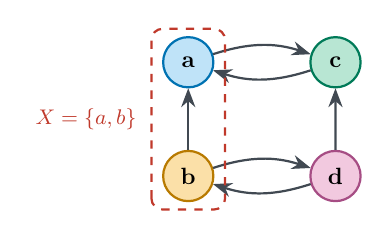
\begin{tikzpicture}[scale=0.85,every node/.style={transform shape}]
  \figtwopref
  \draw[warn,thick,dashed,rounded corners] (-0.55,-0.5) rectangle (0.55,2.2);
  \node[font=\small,text=warn,anchor=east] at (-0.65,0.85) {$X=\{a,b\}$};
\end{tikzpicture}\\[1mm]
{\scriptsize $a\leftrightarrow c$ and $b\leftrightarrow d$ are disjoint cycles, so $\gamma=2$}
\column{0.58\textwidth}
\centering
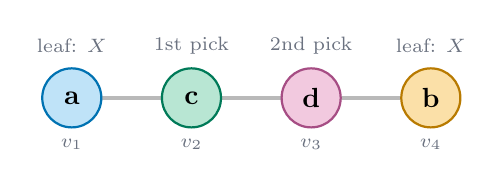
\begin{tikzpicture}[scale=0.95]
  \pathseat{a}{c}{d}{b}
  \seatlabels
  \node[lab] at (0,0.7) {leaf: $X$}; \node[lab] at (4.8,0.7) {leaf: $X$};
  \node[lab] at (1.6,0.7) {1st pick}; \node[lab] at (3.2,0.7) {2nd pick};
\end{tikzpicture}\\[2mm]
\small $c$ (sink) sits by $a$; then $d$. \ Result $a,c,d,b$ is NS.
\end{columns}
\vspace{3mm}
\begin{itemize}
  \item \textbf{Planar} preferences: $\gamma\le\frac35 n$, so any seat graph with $\ge 60\%$ leaves works.
\end{itemize}
\idea{Same trick as colouring games on DAGs: sinks choose first.}
\note{\tm{Achyuth}{0:45}{33:00}
On our running example: the two mutual pairs are disjoint cycles, so we must remove two agents, say $a$ and $b$; $\gamma=2$. A path of four seats has two leaves. Put $a$ and $b$ on the ends. Among $c$ and $d$, $d$ likes $c$, so $c$ is the sink and picks first: it likes $a$, so it sits next to $a$. Then $d$ takes the last seat, next to both $c$ and $b$. We get $a,c,d,b$, the same as the greedy path seating.

Consequence from the paper: planar preference graphs have DFVS at most three-fifths of $n$, so any seat graph that's at least 60\% leaves works, for example full $m$-ary trees with $m$ at least 3.

Course link: this is the same trick as for colouring games on DAGs: let the sinks choose first, in reverse topological order.}
\end{frame}

% ---------------------------------------------------------------- 29
\begin{frame}{Open questions (from the paper)}
\begin{itemize}\setlength\itemsep{5mm}
  \item \textbf{Other seat graphs:} grids, trees, and more conditions in the style of Theorem 4.
  \item \textbf{Efficiency:} how much welfare is lost by insisting on NS? Can we maximise welfare among NS seatings?
  \item \textbf{Beyond yes/no preferences:} on cycles NS can fail with cardinal values; on paths this is still open.
\end{itemize}
\note{\tm{Achyuth}{1:00}{34:00}
To close, the open directions the paper itself lists in its conclusion.

First, other seat graphs: does NS always exist on grids or trees? And more results like Theorem 4 would help describe which instances always have an NS seating.

Second, efficiency: how much total happiness is lost by insisting on NS, the price of neighbourhood stability, or how to find the happiest seating among the NS ones.

Third, richer preferences. On cycles, NS can already fail with cardinal values, as we saw. On paths, the question is open.}
\end{frame}

% ---------------------------------------------------------------- 30
\begin{frame}{Summary}
\begin{itemize}\setlength\itemsep{1.5mm}
  \item \textbf{Neighbourhood stability:} only neighbours can swap. Weaker than stability, and natural.
  \item \textbf{Not always possible:} $K_{t,t}$ with $t$ odd (Theorem 1). Swaps can loop even on 4 seats (Proposition 1).
  \item \textbf{Cycles:} always possible, $O(n^3)$, via path partitions and a progress measure (Theorem 2).
  \item \textbf{Paths:} even distance-2 stability, by a greedy algorithm (Theorem 3).
  \item \textbf{General:} NS exists if the seat graph has enough leaves compared with the DFVS number (Theorem 4).
\end{itemize}
\vspace{4mm}
\begin{center}\Large\bfseries\color{accent} Thank you! Questions?\end{center}
\note{\tm{Achyuth}{0:30}{34:30}
To summarise. Neighbourhood stability only lets neighbours swap; it's weaker than stability and natural for seating. It can fail, on complete bipartite seat graphs with odd $t$, and swap dynamics can loop even on four seats. But on round tables an NS seating always exists and is found in cubic time using path partitions. On benches we even get distance-two stability by a greedy algorithm. And for general seat graphs, having enough leaves compared to the DFVS number suffices.

Thank you, we're happy to take questions.

(Backup if asked: our brute-force scripts checked every 4-agent instance on the 4-cycle and 6,000 random 5--6 agent instances; no counterexample to Theorem 2.)}
\end{frame}

\end{document}
